% !Mode:: "TeX:UTF-8"
% !TEX root = main.tex

\iffalse
\bibliography{reference/reference.bib} % 欺骗latextools获取bib文件
\fi

%%%%%%% 正文 %%%%%%%
\chapter{章节}

\section{部分}

最优化\cite{optim}是数学和计算机科学领域中的一个重要分支,旨在寻找函数的最小值或最大值,以满足一定的约束条件。最优化方法在科学、工程、经济学、物理学、机器学习等领域广泛应用,它们有助于解决各种实际问题,如参数估计、资源分配、模型拟合等。最优化是一个广泛而有挑战性的领域,它在不同领域的应用范围广泛,从优化机器学习算法到优化工程设计都有重要作用。选择适当的最优化方法和合适的工具是解决实际问题的关键。

\begin{figure}[H]
\centering
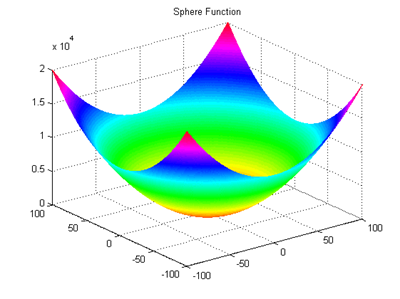
\includegraphics[width=0.75\textwidth]{demo.png}
\caption{Demo}\label{fig:demo}
\vspace{-1em}
\end{figure}


\begin{lstlisting}
import numpy as np
# Your code here
\end{lstlisting}


\begin{table}[H]
\caption{demo}\label{tab:demo}
\vspace{0.5em}\centering\wuhao
\begin{tabular}{cccc}
\toprule[1.5pt]
$n$ & $x$ & $y$ & $f(x, y)$\\
0 & 40.08 & 40.08 & 3213.01 \\
\midrule[1pt]
\bottomrule[1.5pt]
\end{tabular}
\vspace{\baselineskip}
\end{table}


\begin{algorithm}
    $i\gets 10$\;
    \eIf{$i\geq 5$}
    {
        $i\gets i-1$\;
    }
    {
        \If{$i\leq 3$}
        {
            $i\gets i+2$\;
        }
    }
\end{algorithm}


\begin{algorithmic}
    \STATE $i\gets 10$
    \IF {$i\geq 5$} 
      \STATE $i\gets i-1$
    \ELSE
      \IF {$i\leq 3$}
        \STATE $i\gets i+2$
      \ENDIF
    \ENDIF 
\end{algorithmic}


%%%%%%% 结论 %%%%%%%

\addcontentsline{toc}{chapter}{结\quad 论} %添加到目录中
\chapter*{结\quad 论}
    
结论在这里



